\documentclass[12pt]{article}
\usepackage[nottoc]{tocbibind}
\usepackage{graphicx}
\usepackage{float}
\usepackage[sorting=none]{biblatex}
\addbibresource{ref.bib}
\graphicspath{ {./images/} }

\begin{document}
\title{Securitatea și confidențialitatea datelor în contextul aplicațiilor mobile}

\author{Ghimpu Lucian Eduard}
\maketitle

\textsc{Conducător științific}

\textsc{Dr. CZIBULA Istvan, Profesor Universitar}

\newpage

\tableofcontents


\section{Introducere}
\subsection{Introducere}
\subsection{Ecosistemul aplicațiilor mobile}
\subsection{GDPR}

\section{Securitatea și confidențialitatea datelor în contextul aplicațiilor mobile}


\subsection{Autentificarea si înregistrarea}
\newpage
\subsubsection{Ceva introducere *}

Indiferent că vorbim de aplicații web, desktop sau mobile, majoritatea folosesc 
o metodă de autentificare. Auntentificarea șî înregistrarea stau la baza
problematicii securității datelor. În clasamentul OWASP Top 10 din 2017 \cite{owasp-top10-2017}, 
problemele legate de autentificare și gestiunea sesiunii, sunt clasate pe locul 2. Iar în
clasamentul OWASP top 10 Mobile din 2016 \cite{owasp-top10-mobile}, autentificare nesigură
și autorizarea necurespunzatoare sunt clasate pe locul 4, respectiv 6.

Unicitatea aplicaților mobile este dată de faptul că un dispozitiv mobil
poate devenii accesibil oricărui persoane datorită portabilitatii lor. Un dispozitiv mobil
poate fi furat, pierdut sau accesat temporal de o persoană necunoscută fără permisiunea
posesorului. Prin urmare nevoia de un sistem de autentificare robust este mandatorie 
atunci când vorbim de aplicații care gestionează date sensibile (aplicații financiare, sociale,
medicale, etc\dots).

\bigskip

În cadrul aplicațiilor mobile, autentificarea se poate face prin mai multe metode. De la
simpla autentificare prin utilizator și parolă, până la utilizarea de sezori biometrici.
Mitigari clasice precum impunerea unei parole sigure rămân valabile și în 
contextul aplicațiilor mobile.


Pentru alegerea metodei de autentificare trebuie să ne punem în primă instanța următoarele două
întrebări:

\begin{itemize}
    \item Care este scopul aplicației? O aplicație care notifica utilizatorul despre starea meteo poate 
    că nu ar avea nevoie de autentificare prin senzori biometrici. 
    \item Aplicația gestionează date confidențiale? Un exemplu potrivit ar fi o aplicație precum BT pay, care gestionează 
    contul curent al unui utilizatorul,
    se folosește de mai multe metode de autentificare, o dată prin datele de logare, iar apoi
    prin senzori biometrici.
\end{itemize}

După ce ne este clar care este scopul aplicației și cu ce fel de date lucrează, 
putem include una sau mai multe metode de autentificare bazate după următorii
factori:

\begin{enumerate}
    \item Ceva ce utilizatorul știe (parolă, pin etc\dots)
    \item Ceva ce il definește pe utilizator (amprenta, retina)
    \item Ceva ce utilizatorul deține (parole generate temporal)
\end{enumerate}

\begin{figure}[H]
\centering
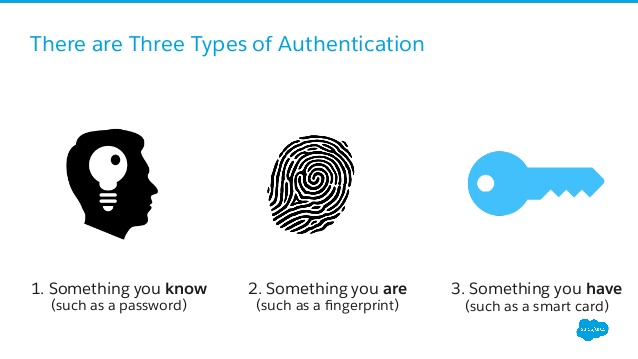
\includegraphics[height=4cm]{3ways.jpg}
\caption{Metode de autentificare \cite{3ways-auth}}
\end{figure}

\subsubsection{JWT}

Majoritatea aplicațiilor de azi se folosesc de cea mai simplă formă de autentificare,
prin folosirea de credentiale (ceva ce utilizatorul știe) și unui token de acces (ceva
ce utilizatorul deține). Utilizatorul își creeza cont pentru o anumită aplicație, folosește
credeințalele pentru a se loga, cererea de autentificare ajunge la server unde se verifică
credențialele iar apoi se generează un token care va fi folosit de utilizator pentru a accesa
diferite resurse în aplicație.

Scenariu descris anterior se referă la folosirea de JWT (JSON Web Token), un standard (RFC 7519) \cite{rfc-7519} 
adoptat de multe aplicații mobile în zilele noastre. 
JSON Web Token este o metodă sigură de autorizare a trasferului
de informații între două părți \cite{jwt}, deobicei 
clientul mobil și serverul la care se face cererea. Clientul revendică de la server
o dovadă, un token, care apoi este folosit de client pentru a accesa diferite 
resurse.

Din punct de vedere tehnic, un JWT are urmatoarea forma 11111.22222.33333 și este
alcătuit din 3 parți:

\begin{enumerate}
    \item Antetul (Header)
    \item Datele utile (Payload)
    \item Semnătura (Signature)
\end{enumerate}


\begin{figure}[H]
    \begin{minipage}[c]{0.5\textwidth}
        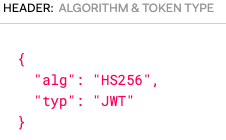
\includegraphics[width=\textwidth]{jwt-header.png}
    \end{minipage}\hfill
    \begin{minipage}[c]{0.5\textwidth}
        \caption{Antetul unui JWT, alcatuit din tipul de algoritm 
        de înregistrare (HS256) și tipul de token (JWT).}
    \end{minipage}
\end{figure}

\begin{figure}[H]
    \begin{minipage}[c]{0.5\textwidth}
        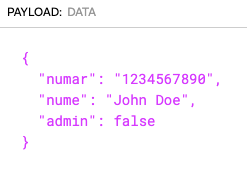
\includegraphics[width=\textwidth]{jwt-payload.png}
    \end{minipage}\hfill
    \begin{minipage}[c]{0.5\textwidth}
        \caption{Partea utilă al unui JWT conține date sau permisiuni
        pe care clientul le are.}
    \end{minipage}
\end{figure}

\begin{figure}[H]
    \begin{minipage}[c]{0.5\textwidth}
        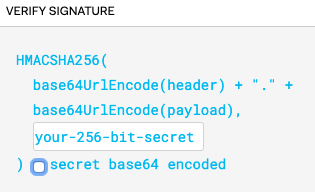
\includegraphics[width=\textwidth]{jwt-sign.png}
    \end{minipage}\hfill
    \begin{minipage}[c]{0.5\textwidth}
        \caption{Semnătura unui JWT este alcătuită din antetul encodat, 
        datele encodate, algoritmul folosit în antet și un secret. Semnătura are rolul
        de a oferi o metodă de verificare pentru a asigura ca conținutul nu a fost 
        modificat }
    \end{minipage}
\end{figure}

\begin{figure}[H]
    \begin{minipage}[c]{0.5\textwidth}
        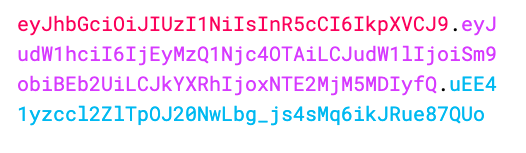
\includegraphics[width=\textwidth]{jwt-all.png}
    \end{minipage}\hfill
    \begin{minipage}[c]{0.5\textwidth}
        \caption{
            JWT va fi format în final 
            de 3 siruri de caractere de tip Base64-URL separate prin punct. }
    \end{minipage}
\end{figure}

O dată ce clientul deține un token, acesta trebuie tratat cu multă grijă 
în cadrul unei aplicații. Acesta poate fi folosit mai apoi în antetul tuturor 
cererilor de tip HTTP sub formă "Authorization: Bearer <token>", din acest motiv 
cel mai probabil se dorește salvarea token-ului în memoria locală a dispozitivului
pentru a putea fi apoi folosit în viitor. Acesta poate fi criptat iar la rândul 
lui la nivelul clientului, deși în mod nativ atât pe android cât și pe ios există metode
sigure de stocare a datelor de tip primitiv (SharedPreferences în mod private pe Android și
keychain pe iOS).

Pentru un nivel și mai mare de siguranță, se poate limita durata de timp
pe care este valabil un token. Spre exemplu aplicația BT Pay folosește un token
care este valid tip de 10-15 minute. După ce token-ul expiră, utilizatorul este nevoit
să se autentifice din nou.

Avantajul principal pe care îl oferă JWT este facilitatea prin care se demarează tot procesul
de revendicare a datelor sau drepturile de la un server de catre client.  
Un alt aspect important îl reprezintă faptul că în spate, totul se produce folosit obiecte
de tipul JSON, fapt ce il face extrem de ușor de implementat și folosit in orice limbaj
de programare.

\subsubsection{Autentificare prin senzori biometrici}

Biometria este termenul tehnic folosit pentru măsurătorile și calculele făcute legate
de corpul uman. Se folosește de metrici legate de caracteristicile umane. În cazul
dezvoltării de software, biometria este folosită pentru autentificare.

Autentificarea prin senzori biometrici se folosește de un factor moștenit, ceva ce îl definește pe
utilizator și prin urmare este una dintre cele mai comode și rapide metode de autentificare.
Mai mult decât atât, datele biometrice precum aprentă sunt greu de furat sau compromis.

Din ce în ce mai multe aplicații încep să folosească autentificare prin senzori 
biometrici, un factor major îl joacă faptul că în ultimi ani, capabilitățile hardware ale
dispozitivelor mobile a crescut exponențial, telefoanele vin încorporate cu diferinti
senzori biometrici precum: senzori de amprenta și recunoaștere facială (iris și rețină).

Metricile biometrice pot varia de la caracteristici fizice pânâ la aspecte ale 
comportamentului unei persoane. În cea ce privește dispozitivele mobile putem idetifica
trei tipuri de autentificari biometrice:

\begin{enumerate}
    \item Senzor de amprentă, extrem de sigur deoarece fiecare individ are
    o amprentă unică.
    \item Recunoașterea vocii, avantajoasă deoarece nu necesitâ hardware in plus dar
    nepotrivit pentru situații unde utilizatorul trebuie să păstreze liniștea.
    \item Recunoaștere facială, la fel ca cea a vocii, nu necesită hardware adițional dar 
    nepotrivit pentru locuri în care luminozitatea este scăzută. 
\end{enumerate}


Utilizarea senzorilor biometrici implică anumite aspecte de care un dezvoltator de
aplicații mobile trebuie să țină cont:

\begin{itemize}
    \item Verificarea ca dispozitivul mobil este încorporat cu senzorii folosiți,
    în cazul în care un dispozitiv nu are senzorii biometrici, dezvoltator trebuie 
    să ofere o metodă alternativă de autentificare. \cite{enisa-2017}
    \item Cererea de permisiunea petru folosirea senzorilor.
    \item Verificarea datele biometrice asociate dispozitivului să nu se modifică
    de la prima autentificare. Această măsură trebuie luată pentru a împiedică cazuri
    în care se adaugă noi date biometrice (amprenta nouă).
\end{itemize}

Deși autentificare prin senzori biometrici este mai rapidă și comodă, această nu ar trebuii
să înlocuiască în mod complet autentificare făcută la nivel de server. 
Ambele metode pot coexista în funcție de context.

\begin{figure}[H]
\centering
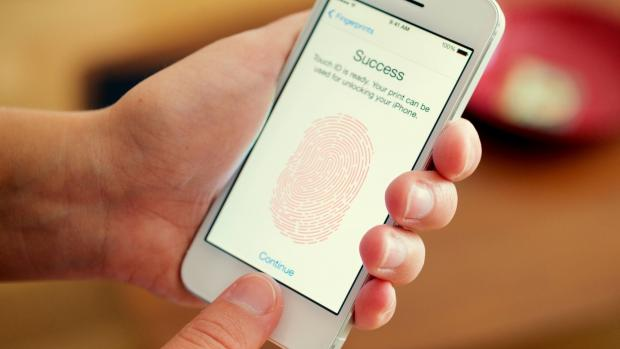
\includegraphics[height=4cm]{fingerprint-smartphone_0.jpg}
\caption{Autentificare prin senzor de amprentă}
\end{figure}

\subsubsection{Autentificare prin factori multiplii}

Autentificare prin factori multiplii (MFA) este un sistem de securizare a autentificării
prin impunerea a mai multor metode de verificare a identității unui utilizator.

Autentificare prin factori multiplii combină mai multe metode independente de autentificare.
Așa cum am văzut în capitolul anterior, autentificarea prin senzori biometrici și autentificarea
prin credentiale lucrează cel mai bine împreună. Pe această idee, rolul autentificării prin factori
multiplii este acela de a creea un sistem greu de compromis în vederea asigurării siguranței și
confidentialitații datelor utilizatorului. Astfel dacă unu din componentele sistemului este compromis,
atacatorul este oprit de restul barierelor. În cazul în care cineva are acces la credentialele unui 
utilizator și la dispozitivul sau mobil, atacatorul poate fi oprit prin folosirea senzorului de amprenta.

Un alt caz de utilizare al autentificarii prin factori multiplii îl reprezintă autentificarea în doi pași
sau OTP (one time password). Rolul autentificarii în doi pași este acela de a crea o barieră în plus
în sistemul de securizare al autentificarii prin creeare de coduri/parole temporare unice.

După ce un utilizator se loghează folosind credențialele valide, un cod unic și temporar este generat
și trimis utilizatorului prin diferite canale, deobicei prin SMS, email sau aplicații special făcute
pentru generarea de coduri unice. Utilizatorul este apoi nevoit să introducă codul primit pentru
a își confirmă identitatea. Utilizarea sa nu se limitează doar la autentificare, ci poate fi folosită în
mod general pentru a confirmă identitatea persoanei. Un exemplu îl reprezintă aplicațiile financiare care
atunci când se încearcă o plata, vor trimite un cod unic pentru a verifică identitatea persoanei care 
a inițiat acțiunea.

Deși folosirea autentificarii prin doi pași este destul de comună în cadrul aplicațiilor mobile, această metodă
prezintă și anumite vulnerabilități, mai ales când canalul de comunicare a parolei este prin SMS sau prin 
apel telefonic.
SMS-urile pot fi interceptate și redirecționate, la fel și apelurile telefonice. În astfel de cazuri
se poate limita valabilitatea codului primit la un iterval scurt de timp (5-10 minute). 

Utilizarea unui sistem de autentificare multiplu precum autentificare în doi pași este de altfel recomandată
și de ENISA \cite{enisa-security-data-processing} într-un studiu făcut în vederea 
siguranței procesării datelor personale de către companii mari.

\begin{figure}[H]
\centering
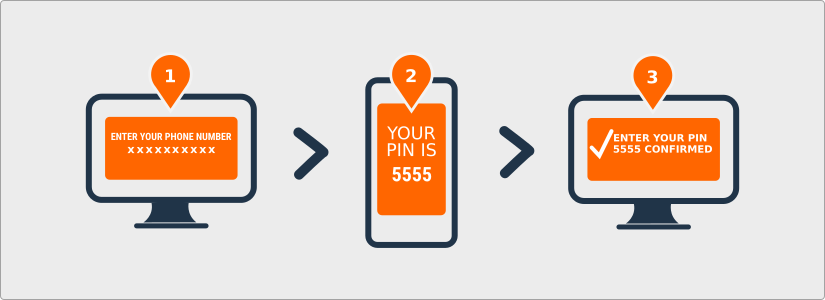
\includegraphics[height=4cm]{wordpress-two-factor-authentication.png}
\caption{Autentificare în doi pași}
\end{figure}

\subsection{Canale de comunicare}
\subsubsection{HTTP și HTTPS}

Majoritatea aplicațiilor mobile se folosesc de unul sau mai multe servere pentru a își aduce date
sau pentru a prelucra date preluate de la utilizator. Această practică este folosită pentru a evita  stocarea de
date pe dispozitivele utilizatorului având în vedere memoria limitată pe care o dețin. Din acest motiv 
este necesar folosire unor protocoale de comunicare. Cele mai folosite protocoale de comunicare în ecosistemul
mobil sunt HTTP și HTTPS.

Aceste protocoale de comunicare sunt un set de reguli care descriu modalitatea prin care datele sun trimise și 
primite. În mediul mobil, HTTP și HTTPS sunt cele maifolosite protocoale pentru a trimite text imagini și sunete.

HTTPS este varianta sigură a lui HTTP, pe tot parcursul comunicării, datele sunt criptate de la un capăt la altul.
Deși HTTP este mai frecvent folosit, este recomandată folosirea protocolului HTTPS mai ales pentru aplicații 
care gestionează date sensibile.

Dezavantul folosirii protocolului HTTPS îl reprezintă performanță. Criptare și decriptarea datelor trasmise sunt
operații costisitoare. Deși există o pierdere de performanță, există studii \cite{goldberg1998comparison} care demonstrează
că diferența de performanță este modestă, și încurajează folosirea protocolului mai sigur. Un alt studiu \cite{felt2017measuring}
arată că pe anumite sisteme de operare mobile, precum Android, rata de adopție pentru HTTPS este în urmă față de rata de adopție
pe desktop. 

\begin{figure}[H]
\centering
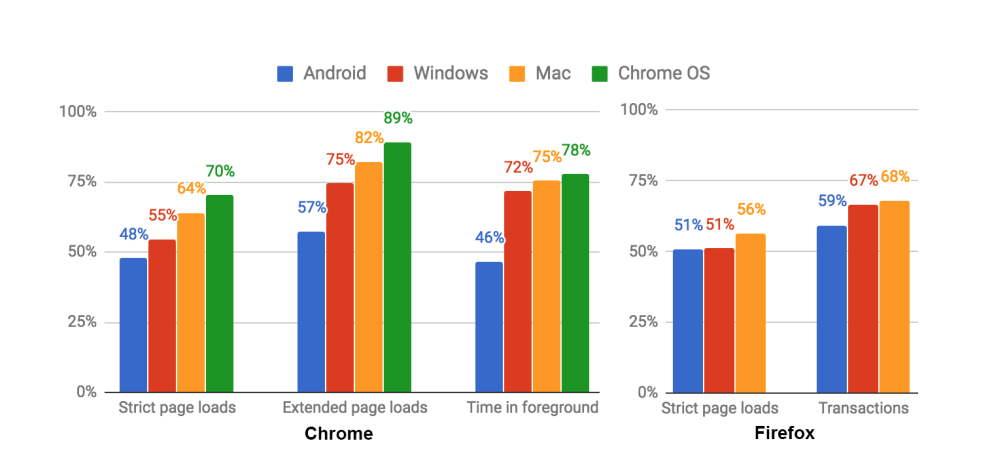
\includegraphics{http.png}
\caption{Procentul de utilizare HTTPS pe diferite sisteme de operare la sfarsitul unei saptamani din
Febraruie 2017 \cite{felt2017measuring}}
\end{figure}

\subsubsection{SMS}

SMS (Short Message Service) este un serviciu folosit de majoritatea dispozitivelor mobile. Cazurile de 
utilizare ale serviciului variază de la simpla folosire pentru a comunica mesaje scurte, până la 
autentificare cu parolă unică. În 2010, 6.1 trilioane de mesaje au fost trimise cu o medie de 193.000 de SMS-uri
pe secundă \cite{riseof3g}. 


Din punct de vedere tehnic, SMS este un protocol de comunicare care permite schimbul de mesaj scurte. Un SMS 
poate fi format din 160 de caractere alfanumerice, mesajele mai mari de 160 de caractere sunt sparte în 
mai multe mesaje. 
Un mesaj trimits este mai întâi interceptat de SMSC (Short Message Service Center) care de cele mai multe ori
este menținut de providerii de rețele telefonice. SMSC-ul trimite mai apoi mesajul către un alt SMSC (al receptorului)
mesaj pe care în final îl trimite receptorului.

În ciudat popularității sale, comunicare prin SMS prezintă
anumite vulnerabilități. Cel mai periculoasă vulnerabilitate 
este "SMS spoofing". Aceasta are loc când un atacator manipulează
adresa mesajului pentru a impersona pe cineva. Aceste tipuri de
atacuri pot fi prevenite prin verificarea datelor emițătorului 
înainte că mesajul să ajungă la receptor. O altă metodă de protejare,
adoptată mai ales în cadrul autentificării prin 2 pași, este folosirea unui
SMS gateway, servicii special dedicate pentru astefel de operații, dotate
cu diverse măsuri de protecție.

\subsubsection{WebSocket}

Standardizat în 2011 în RFC 6455 \cite{fette2011websocket}, WebSocket este
un protocol de comunicare bidirecțional bazandu-se defapt o conexiune de tip TCP.

Principalul avantaj pe care îl oferă protocolul WebSocket este facilitatea
prin care se permite trasferul de date în mod bidirecțional. În comparație cu protocolul HTTP,
un server poate transmite date unui client fără ca acesta să fie făcut o cerere.

La fel ca HTTP, protocolul WebSocket (WS) este dublat de variată protejată WSS, oferind
criptare de la un capăt la altul al comunicării.

Când vine vorba de aplicații mobile, WebScocket-urile sunt folosite
predominant de aplicații care au nevoie de o comunicare de tip broadcast. 
Aplicațiile de mesagerie în grup precum WhatsApp folosesc WebSocket-uri pentru
a notifica toți utilizatorii unui grup de mesajele noi primite.

Deși WebSocket rezolvă probleme de conectivitate, nu rezolva și problemele de 
securitate \cite{erkkila2012websocket}. vulnerabilități la nivelul acestui protocol
variază de la simple interceptări ale datelor în rețea, atunci când se folosește varianta
neprotejată a protocolului, până la vulnerabilități mai severe precum blocarea serviciului
(DDos) \cite{test-ws}. Pentru a evita astfel de probleme este sugerată folosirea variantei
protajate (wss) și limitarea conexiunilor sau verificarea conexiuniilor când provin din aceasă sursă.


Fiind o tehnologie încă tânăra, WebSocket încă nu este la fel de răspândit
precum HTTP sau SMS, dar că orice sistem de comunicare, includerea lui într-o
soluție soft necesită atenție sporită pentru a prevenii eventuale probleme de securitate.


\subsection{Persistența datelor}
\subsubsection{Metode de persistare a datelor}
\subsubsection{Criptografie}
\subsubsection{Gestionarea datelor sensibile}

\subsection{Alți factori}
\subsubsection{Permisiuni}
\subsubsection{Webviews}
\subsubsection{Distribuirea aplicației}
\subsubsection{Probleme specifice pe anumite platforme}

\section{Medicarium}
\subsection{Analiza aplicației}
\subsubsection{Problematica}
\subsubsection{Cazuri de utilizare}

\subsection{Proiectarea aplicației}
\subsubsection{Arhitectura}
\subsubsection{UML ceva???}

\subsection{Implementarea aplicației - Serverul și serviciile}

\subsubsection{Server REST}
\subsubsection{Node.js}
\subsubsection{MongoDB}
\subsubsection{Rute disponibile}
\subsubsection{Autentificare in doi pași}

\subsection{Implementarea aplicației - Clientul mobil}
\subsubsection{Android Jetpack}
\subsubsection{Kotlin}
\subsubsection{Autentificarea}
\subsubsection{Securitatea aplicației}
\subsubsection{Gestionarea permisiunilor}
\subsubsection{Gestionarea fisierelor}

\subsection{Testarea}

\section{Manual de utilizare}

\section{Concluzii}

\newpage

\section{Bibliografie}
\nocite{owasp-top10-2017}
\nocite{owasp-top10-mobile}
\nocite{3ways-auth}
\nocite{rfc-7519}
\nocite{jwt}
\nocite{enisa-2017}
\nocite{enisa-security-data-processing}
\nocite{goldberg1998comparison}
\nocite{felt2017measuring}
\nocite{fette2011websocket}
\nocite{erkkila2012websocket}
\nocite{test-ws}
\printbibliography[title=Bibliografie]

\end{document}